
The central component of the work scope is the development of robust low-cost
ROMs for reactor thermal design and analysis.  ROMs typically comprise a small
system of ordinary differential equations (ODEs) that represent the evoluton of
$N \approx 100$ basis functions designed to capture the dominant dynamics of
the flow field.  For this size, the low-dimensional ODE (\ref{eq:eromd}) can
   be advanced extremely fast---\textbf{in just a few minutes on a laptop it is
   possible to evolve tens-of-thousands of convective time units,} much longer
   than feasible with a high-fidelity simulation, even on an exascale platform,
   which is one of the reasons that ROMs are interesting for long-time transients.  
{\em Parametric model order reduction} (pMOR) is a process through which
a ROM or suite of ROMs is constructed to estimate the system behavior 
over a range of parametric inputs (e.g., inlet flow rates, thermal loading,
or Reynolds number)
without the need for high-fidelity simulations at every point in the target
parameter space.  The output of the pMOR will be a small set of coefficients to
drive low-rank systems of ODEs that can be directly coupled with either a
Systems Analysis Module (SAM) or with detailed, localized, LES or RANS models.

The ROMs are based on data (solution snapshots) from high-fidelity direct
numerical (DNS), large-eddy (LES), or unsteady Reynolds-averaged Navier-Stokes
(uRANS) simulations of turbulent thermal transport.   These \textit{full-order
models} (FOMs) will be run on DOE's leadership computing facilities in an {\em
offline} mode using the NEAMS-supported Nek5000/RS code developed by the PIs.
(NekRS is the GPU-oriented version of Nek5000, developed under the DOE's
Exascale Computing Project.) The ROMs will be used in a real-time {\em online}
mode simulating the governing Navier-Stokes and energy equations as a
projection of $N$ basis functions derived from a
proper-orthogonal-decomposition (POD) of snapshots generated by the FOMs.

There are three essential categories for the proposed ROM development:
\textit{i. The reproduction problem}, in which the ROM is able to
adequately reproduce a given quantity of interest (QOI), such as
flow rate or Nusselt number, over the same time period and at the
same parameter points as the originating FOM data;
\textit{ii. The parametric problem}, in which the ROM is used to
to predict QOIs at a {\em different} point in parameter space;
and
\textit{iii. Long time transients}, in which the ROM is used to
predict QOI behavior beyond the sampled time-domain of the FOM.
Categories \textit{ii} and \textit{iii} bring their own challenges
(e.g., \cite{tsai22a}) but they depend crucially on having a 
stable and accurate ROM for turbulent flows, which is an open
research question and a major focus of our Category \textit{i} effort.
If the ROM is stable and accurate, then Category \textit{iii} is 
effectively similar to \textit{ii} since the time window can be
viewed as a parameter.

  Under NEUP Award 18-15520, we have developed NekROM to provide a pMOR/ROM
capability within the Nek5000/RS framework that allows users to build ROMs and
perform parameter variation with these models.  The analysis process begins
with a detailed FOM of size (number of degrees-of-freedom)
$\cN=10^7$--$10^{11}$ and $K \approx 10^3$ snapshot files.  The NekROM software
module then distills the FOM results into a ROM ODE system of size $N \approx
100$, which can be solved with a choice of Fortran, Matlab, or Python drivers
in the NekROM suite.  An outer driver is provided to iterate between the ROM
and Nek5000/RS to pick optimized (error-indicated) anchor (trial) points in the
target parameter space, $\cP$.
  The principal focus of this project will be to push the \textbf{state-of-the-art} 
for ROM-based simulations of turbulence, to identify which turbulence problems are
tractable, and which are not \cite{tsai22a}, to integrate the ROM simulator with
the RANS and LES capabilities in Nek5000/RS, and to test this multiscale 
framework within a suite of TH challenge problems described in the next section.


%% will be on developing ( \textit{ii.}-- \textit{iv.}), supported by
%% simulations with Nek5000/RS (\textit{i.}), which is well-established as a scalable
%% code for solving the full-order models (e.g., \cite{merzari11b,merzari15a,sc22}). 

%% Realization of a viable analysis tool requires economization of costs at all
%% stages of the process, including a reduction in the number of expensive
%% offline simulations and a reduction in the size of the
%% reduced-basis sets $N$, which incur costs scaling as $O(N^3)$ because 
%% of the nonlinear interactions in the Navier-Stokes equations.
%% In addition to costs, stability and accuracy of the ROM are also critical.
%% 
%%   To address these concerns, the proposed methodology will expand upon recent
%% developments in ROMs for long-time simulations of turbulent flows outlined in
%% \cite{fick18}.  Key ingredients of this approach are:
%%  \textit{i.} $H^1_0$-POD-based basis sets for unsteady turbulent flows
%%          at fixed anchor points $\cP_{\mbox{\tiny anch}}$ in the target
%%          parameter space, $\cP$;
%%  \textit{ii.} a novel constraint-based stabilization of the ROM derived
%%           from the full-order models;
%%  \textit{iii.} effective dual-norm error estimates that {\em inexpensively}
%%            indicate the model error at any point in $\cP$; and
%%  \textit{iv.} an efficient greedy algorithm for optimizing the choice of
%%           anchor points to meet the desired model error tolerance 
%%           for any point $\up^* \in \cP$.
%% We remark that the error estimators are essential to an efficient POD
%% formulation of this problem and are a {\em unique} contribution of the proposed
%% approach.  The constraint-based stabilization of the ROM is also {\em unique}
%% to the proposed effort.  This project will provide the first tests of this
%% approach in industrially-relevant settings.   
%% 
%% 
%% \noindent
%% {\bf High-Fidelity Simulations on DOE Leadership Computers.}
%%   DOE's current- and next-generation leadership computers employ nodes that
%%   feature high-performance GPUs.
%% We have recently demonstrated that it is possible to simulate a single
%% flow-through time for the thermal-hydraulics of a full pebble-bed reactor core
%% (352,000 pebbles) in just six hours of wall-clock time on using 27648
%% NVIDIA V100s on ORNL's Summit \cite{sc22}.  This is an significant acheivement
%% as it involves updating a quarter-trillion degrees-of-freedom at $\approx$ 0.3
%% seconds per step.  The software that enables this achievement is {\em NekRS},
%% which is the GPU-oriented version of the highly-scalable thermal-fluids code,
%% Nek5000.
%% %% NekRS is being developed under DOE's Center for
%% %% Efficient Exascale Discretizations (CEED) and
%% NekRS sustains $\approx$ 0.5--1.0 TFLOPS ($10^{12}$
%% floating point operations per second) per MPI rank on current pre-exascale
%% platforms and 80\% parallel efficiency at about 2M grid points per rank.
%% Consequently, a 51B grid-point problem such as the pebble-bed reactor of Fig.
%% \ref{fig:sum}(right) can effectively use $P$=25,000 GPUs. While such a calculation
%% fills all of Summit, it will require only a fraction of DOE's exascale
%% platforms, where we can anticipate running much larger problems, or running at
%% multiple points in the reactor design space.
%% 
%% Like Nek5000, NekRS is based on high-order spectral element
%% discretizations that have minimal dispersion and dissipation, which
%% are essential features for simulation of turbulence.  Time-stepping
%% uses either a $k$th-order semi-implicit method ($k$=2 or 3) or a
%% characteristics scheme that allows Courant numbers $>$ 1.
%% Fast Poisson solvers are critical to rapid simulation of reactor flows.
%% NekRS has an extensive suite of preconditioners for the pressure-Poisson
%% problem that are tailored to accelerator-based HPC platforms.  NekRS supports
%% most of the features of Nek5000, including a large variety of boundary
%% conditions and extensive tools to analyze turbulent heat transfer.
%% 
%% 
%% 
%% % \begin{figure}[t!] \centering
%% %     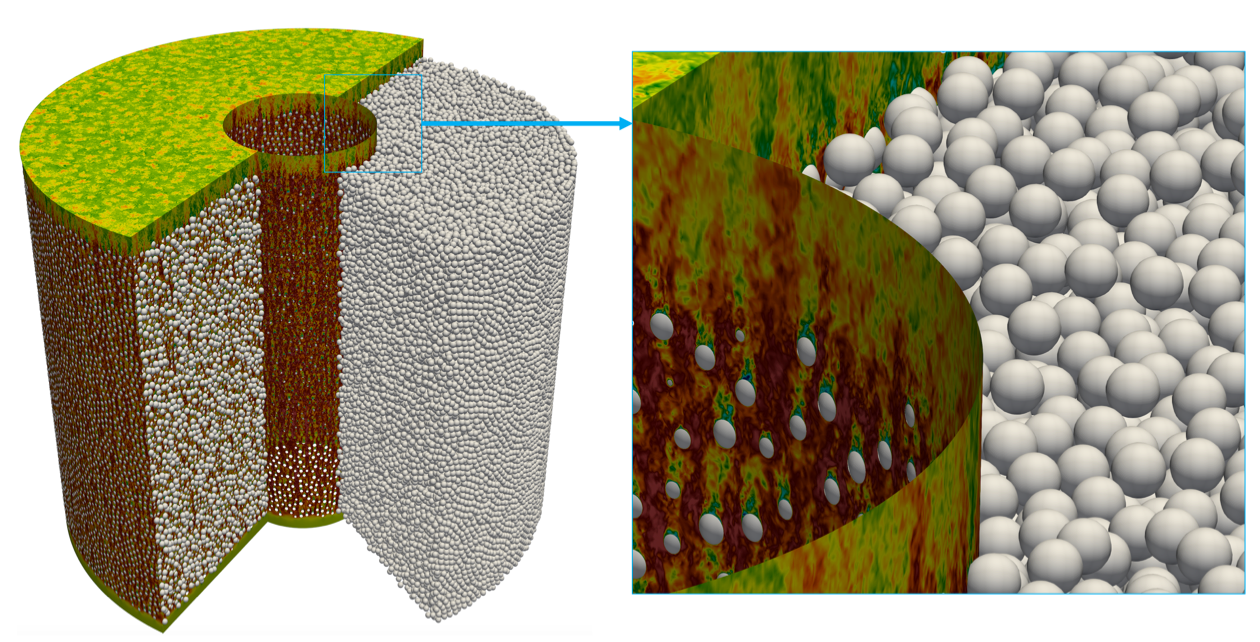
\includegraphics[width = 0.60\textwidth]{figs/pbr_pair.png}
%% %     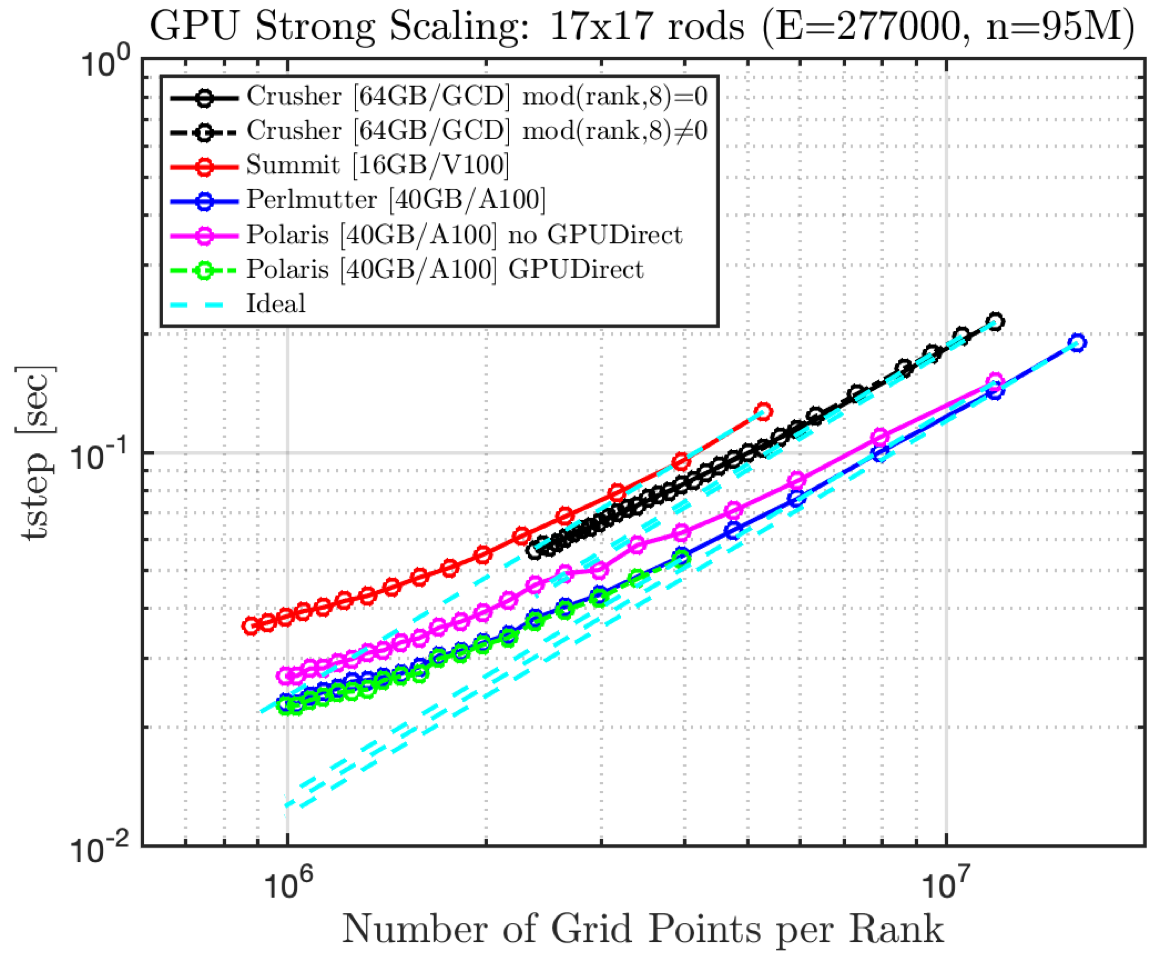
\includegraphics[width = 0.35\textwidth]{figs/nekrs_17x17_crusher_strong.png}
%% %     \caption{(left)
%% % NekRS turbulent flow simulation results for a full reactor core with 352625
%% % pebbles. The simulation comprises 51 billion gridpoints and requires 0.36
%% % seconds per step, which corresponds to six hours for a single flow-through time
%% % on all of Summit.  (Computation by Yu-Hsiang Lan, ANL/UIUC \cite{sc22}.)
%% % (right) NekRS strong-scaling on current-generation accelerator-based platforms:
%% % AMD-MI250X-based Crusher (OLCF),
%% % NVIDIA-V100-based Summit (OLCF),
%% % NVIDIA-A100-based Perlmutter (NERSC),
%% % NVIDIA-A100-based Polaris (ALCF).
%% % The test problem is a 17$\times$17 rod-bundle with 95 million grid points.
%% % (Simulations by Misun Min, ANL, and Yu-Hsiang Lan, ANL/UIUC.)
%% % \label{fig:pbr}}
%% %\end{figure}
%% 
%% 
%% %% (WHY ROM)
%% \noindent
%% {\bf Data-Driven Reduced-Order Models.}
%% While it is clear that NekRS will be capable of delivering fast turn-around
%% for reactor-scale simulations on DOE's exascale platforms, the use of
%% such simulations for one-off determination of system behavior at a single
%% parameter point does not fully leverage the data generated by such large
%% calculations.
%% From a design perspective, it is far more efficient if one can reliably
%% explore parametric input/output relationships (e.g., Nusselt/Rayleigh-number
%% relationships under low-flow conditions) in the neighborhood of the parameter
%% space for which the high-fidelity DNS or LES is performed.   Such a capability
%% is precisely the goal of parametric model-order reduction (pMOR), which is
%% typically based on reduced-order models (ROMs) of the high-fidelity DNS/LES
%% (often referred to as full-order models, or FOMs).
%% 
%% We begin with the reproduction problem. The standard approach is to use
%% $K$$\approx$1000 high-fidelity solution snapshots (i.e., full velocity/temperature
%% fields) to form $N$$\approx$20--200 basis functions through
%% proper-orthogonal decomposition (POD) or some other low-rank approximation
%% approach.  These bases can be used to approximate solutions to the governing
%% Navier-Stokes and energy-transport equations, from which one can extract a
%% low-dimensional dynamical system governing the unknown basis coefficients.
%% These systems, which are of size $N$, run extremely fast---{\bf in just a few
%% minutes on a laptop it is possible to evolve tens-of-thousands of convective
%% time units,} much longer than feasible with a FOM, even on an exascale platform,
%% which is one of the reasons that ROMs are interesting for long-time transients.
%% Moreover, it is relatively easy to adjust equation parameters to have a nominal
%% pMOR tool.
%% %  (Adjusting geometry is more challenging and one of the
%% %  topics to be explored in the context of this project).
%% 
%% \begin{figure}[t] \centering
%% {\setlength{\unitlength}{1.0in}
%%  \begin{picture}(6.5,1.40)(0,0.05)
%%  \put(-.08,0.15){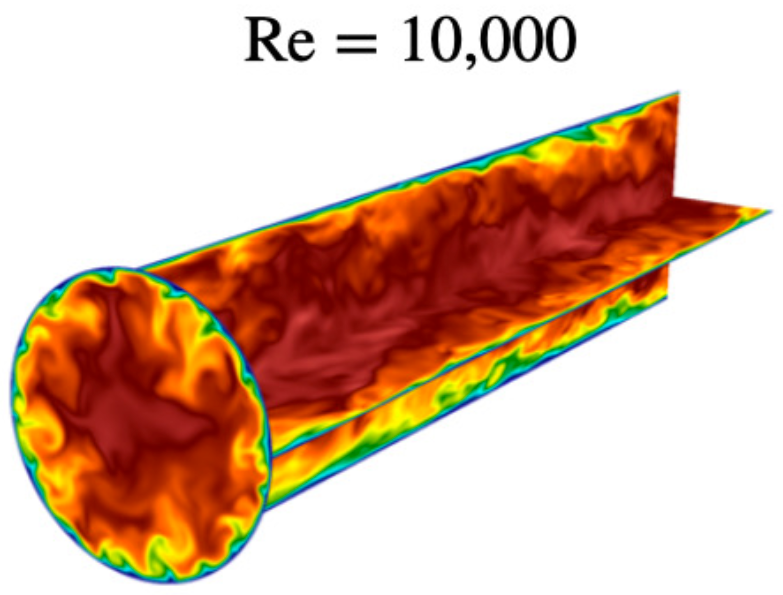
\includegraphics[width = 0.24\textwidth]{figs/kaneko_diss_pipe_r10k.png}}
%%  \put(1.75,0.00){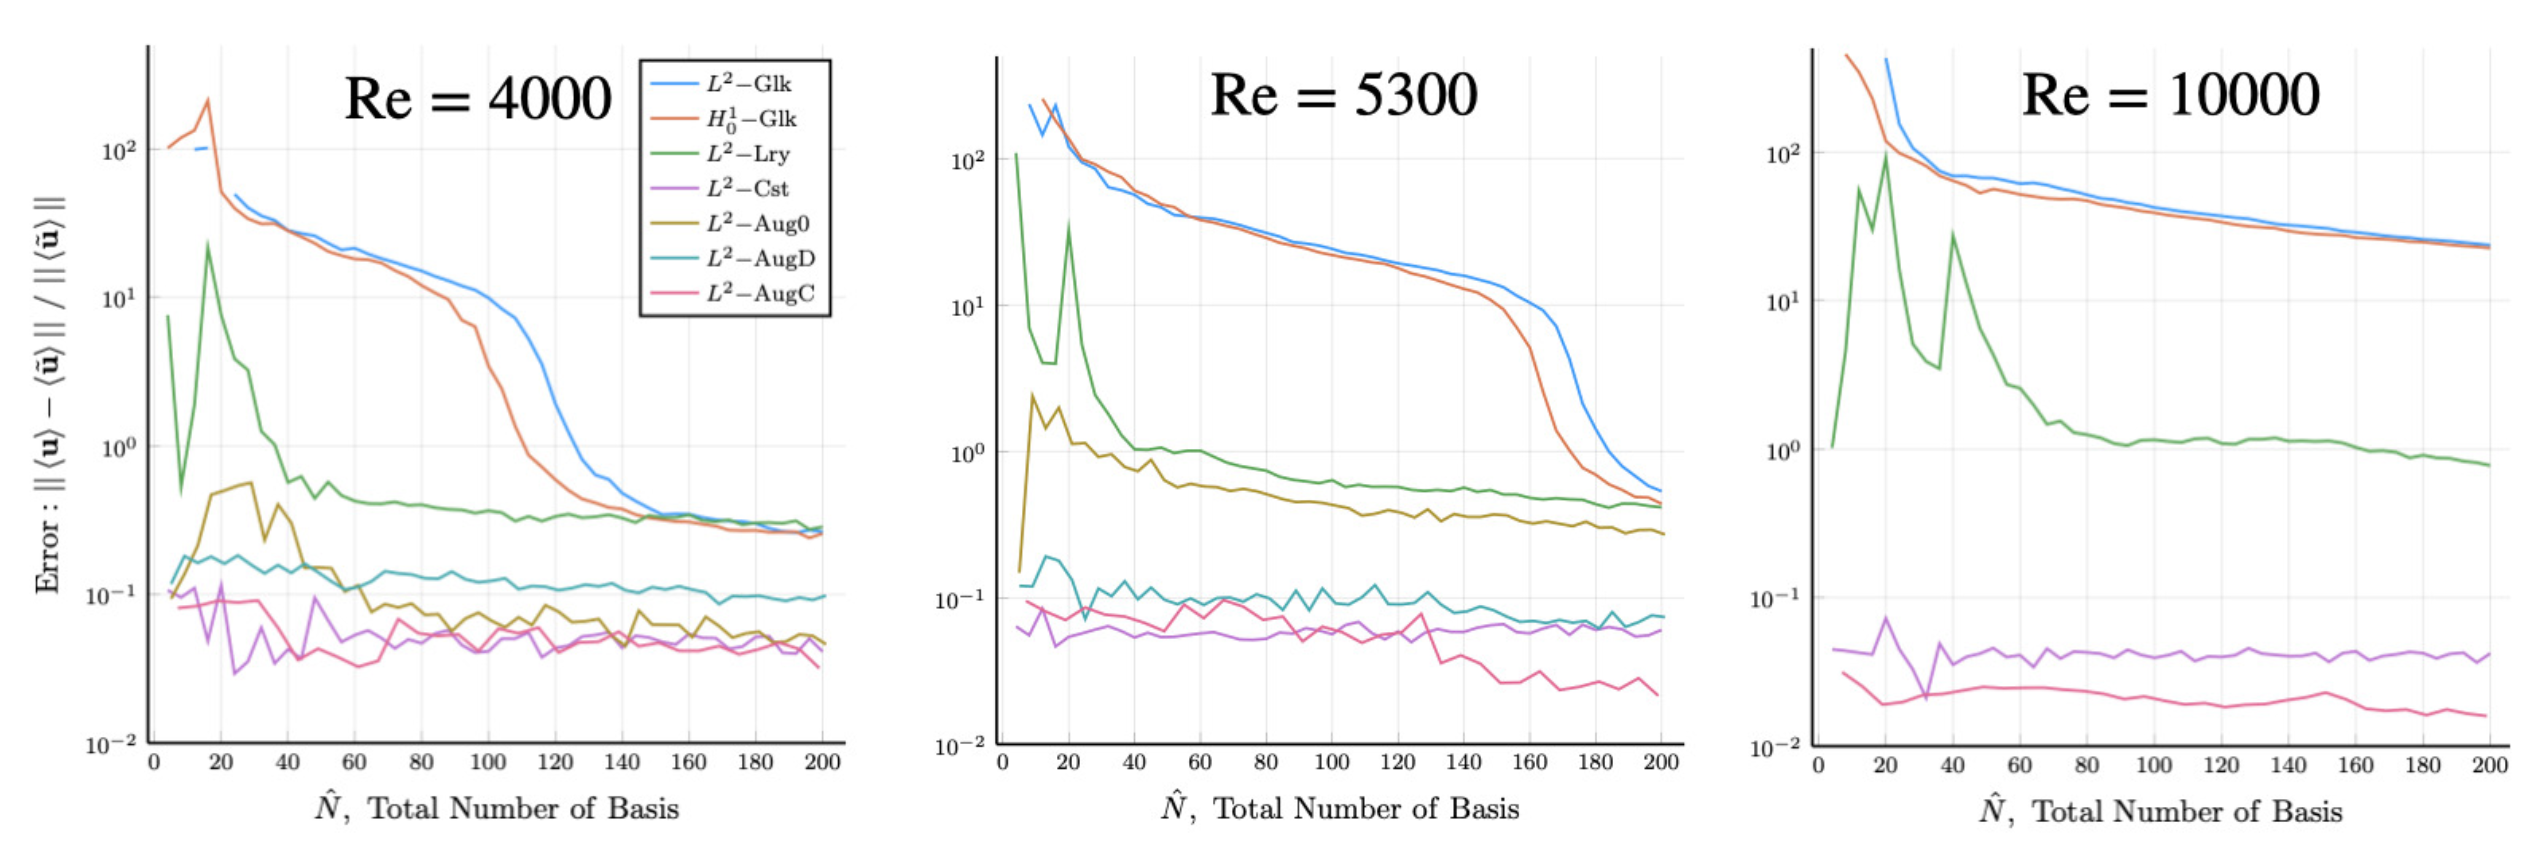
\includegraphics[width = 0.70\textwidth]{figs/kaneko_diss_pipe_ubar.png}}
%% \end{picture}}
%% \caption{
%% {\bf (left)}
%%     Nek5000 DNS of turbulent pipe flow at $Re_D$=10,000;
%% {\bf (right)}
%%     Mean velocity error in ROM reproduction results for
%%     Galerkin POD ($L^2$-Glk, $H^1$-Glk),
%%     Leray- and constrainted-based regularization
%%     ($L^2$-Lry, $H^1$-Cst), and
%%     ABM with three different subsets of the nonlinear terms
%%     ($L^2$-Aug0=$\bz_0 \cdot \nabla \bz_j+ \bz_j \cdot \nabla \bz_0$,
%%     $L^2$-AugD=$\bz_j \cdot \nabla \bz_j$,
%%     $L^2$-AugC=$L^2$-Aug0 $\bigcup$ $L^2$-AugD) \cite{kaneko22a,kaneko22}.
%% \label{fig:abm}}
%% \end{figure}
%% 
%% 
%% There are several challenges to bringing the preceding scenario to fruition.
%% The first is to ensure that the ROM can accurately track the quantities
%% of interest (QOIs) produced by the FOM, even at the same parameter point.
%% Accuracy is by no means assured, particularly for turbulent flows
%% where energy is dissipated by small-scale structures that are generally absent
%% from POD bases.  Several stabilization strategies are possible, such as Leray
%% regularization \cite{wang2012proper} or constrained coefficient evolution
%% \cite{fick18}.  Alternative approaches include modification of the approximation
%% space.  For example \cite{akkari19} uses a decomposition of modes
%% into distinct sets minimizing the $L^2$ error (for accuracy) and the $\cH^1$
%% error (for stability).  In \cite{khodkar2019}, a basis is derived from Green's
%% functions approximations.
%%    Under prior NEUP support, Kaneko \cite{kaneko22a,kaneko22} developed an
%% augmented-basis method (ABM) wherein a set of standard POD basis functions,
%% $\{\bz_i(\bx) \}$,  is augmented with a subset of their nonlinear interaction
%% terms, $\{\bz_i \cdot \nabla \bz_j\}$.
%%   The success of the ABM is illustrated in the turbulent pipe flow
%% examples of Fig. \ref{fig:abm}, which shows that standard POD Galerkin and
%% Leray regularization can converge at lower Reynolds numbers $Re$ with a
%% sufficient number of basis functions, $N$, but that the required number of
%% basis functions rapidly increases with $Re$.  Given the $O(N^3)$ costs for the
%% ROM, these methods are limited to relatively low $Re$.  The ABM and
%% the constrained approaches, however, perform much better because of their
%% stability.  The turbulent kinetic energy behavior is similar to the
%% mean velocities shown in Fig. \ref{fig:abm}, but the ABM
%% can be overly dissipative at higher $Re$.  The mechanism for this anomalous
%% behavior is under investigation.
%% 
%% \begin{wrapfigure}{rt}{3.2in} \centering
%%    {\setlength{\unitlength}{1.0in} \begin{picture}(3.000,1.850)(0.05,.14)
%%      \put(0,0.00){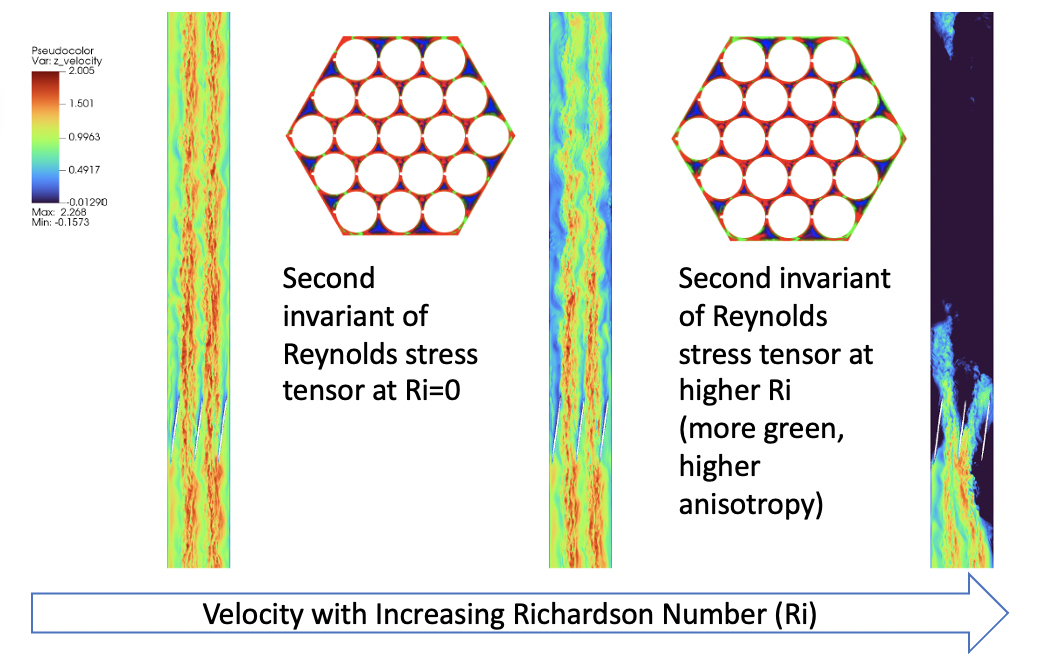
\includegraphics[scale=0.43]{figs/challenge.png}}
%%    \end{picture}}
%%    \caption{Velocity distribution in wire-wrapper assembly as a function of
%%     the Richardson number at low flow conditions. \label{fig:cha}}
%% \end{wrapfigure}
%% With a robust reproduction capability, the next step in pMOR is to ensure that
%% the ROM can accurately predict the system behavior at other parameter points
%% and, ideally, provide error indicators to assess the departure between the ROM
%% and the FOM.  As a step toward pMOR for 3D reactor analysis, under NEUP
%% 18-15520,  we extended the error-estimators of \cite{fick18} to develop
%% an error-indicated pMOR for high Rayleigh-number two-dimensional slot
%% convection in \cite{tsai22a}.
%% By using a greedy algorithm, the error indicators allow one to optimize
%% construction of a parametric map in which new FOMs are run wherever
%% discrepancies between the ROM and FOM are deemed to be large.
%% In \cite{tsai22a}, we also identify chaotic FOMs where certain QOIs are not
%% reproducible either by a ROM or a FOM.
%% 
%% \noindent {\bf Challenge Problem.}
%% Fluid flow and heat removal through fuel, shield and reflector assemblies  can
%% have major impacts on operation and safety for Sodium Fast Reactors (SFRs).
%% This type of reactor is of great interest in the United States due to the
%% planned  deployment of Terrapower's Natrium concept funded partially through
%% the Advanced Reactor Demonstration program (ARDP). These assemblies are formed
%% by bundles from 19 to 217 pins, with a wire wrapped around each pin to maintain
%% the rods in place.
%% 
%% During transients, these assemblies are characterized by a range of conditions
%% that result from reduced flow rates and from large-scale organized flow
%% patterns, including potential intra-assembly buoyancy-driven circulation. Such
%% low flow cases can provide challenges for experiments due to complications in
%% measuring the flow rates and temperatures with high accuracy in different
%% areas. This consequently also raises the uncertainty of many modeling
%% approaches for these phenomena, where existing correlations and sub-channel
%% methods fail. An example of the complex range of flow patterns in provided in
%% Fig. \ref{fig:cha}, which shows a transition from steady forced convection to
%% mixed convection.  Massive circulations are introduced: in a realistic
%% transient the bundle will encounter the full range of conditions. We ultimately
%% seek methods that can provide accurate and \textit{predictive} results.
%% 
%% % \begin{figure}[t!] \centering
%% %     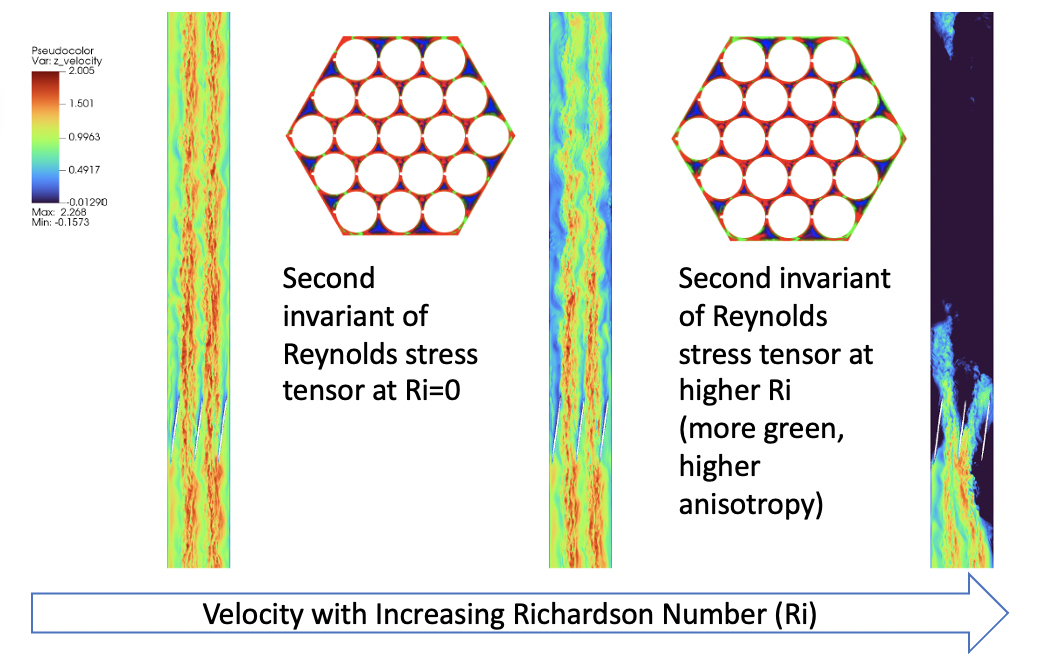
\includegraphics[width = 0.50\textwidth]{figs/challenge.png}
%% %     \caption{ Velocity distribution in wire-wrapper assembly as a function of
%% %     the Richardson number at low flow conditions. \label{fig:cha}}
%% % \end{figure}
%% 
%% 
%% 
%% 
%% \input tex/proposed
